\chapter{Problem 3 - Service-to-Service Authentication \& Trust}

\section{Rancangan Solusi}

\subsection{Otentikasi dan Otorisasi antar Servis}

\textbf{Flow PVMBG:}

\begin{enumerate}
\def\labelenumi{\arabic{enumi}.}
\tightlist
\item
  PVMBG menyediakan layanan untuk mengakses \emph{resource protected} mereka. Perlu daftar akun terlebih dahulu.\\
\item
  Setelah daftar akun dan mengisi beberapa data berkaitan dengan instansi/perusahaan untuk memverifikasi penggunaan, admin PVMBG akan memverifikasi pendaftaran.\\
\item
  Apabila sudah terverifikasi, BNPB akan mendapat client ID dan client secret.\\
\item
  Setelah client ID dan client secret didapatkan, BNPB \emph{generate} one time code (misalnya melalui web interface PVMBG) agar bisa mendapat access token untuk pertama kalinya:
\end{enumerate}

\begin{longtable}[]{|>{\raggedright\arraybackslash}p{\dimexpr(\linewidth-4\tabcolsep)/2\relax}|>{\raggedright\arraybackslash}p{\dimexpr(\linewidth-4\tabcolsep)/2\relax}|}
\hline
\texttt{URL} & \texttt{/oauth/token} \\
\hline
\endhead
\endlastfoot
\texttt{Method} & \texttt{HTTP\ POST} \\
\hline
\textbf{\texttt{Header}} & \\
\hline
\texttt{Authorization} & \texttt{Basic\ Y2xpZW50X2lkOmNsaWVudF9zZWNyZXQ=} \\
\hline
\textbf{\texttt{Request\ Body}} & \\
\hline
\texttt{code} & \texttt{\textless{}one\_time\_code\textgreater{}} \\
\hline
\texttt{grant\_type} & \texttt{authorization\_code} \\
\hline
\end{longtable}

Dengan authorization header bernilai \textless client\_id\textgreater:\textless client\_secret\textgreater{} dalam format base64

Akan dikembalikan:

\begin{codebox}
{
    "access_token" : "<access_token>",
    "refresh_token" : "<refresh_token>",
    "expires_in" : 60
}
\end{codebox}

Dengan ketentuan bahwa access token yang dipakai oleh service BNPB untuk mengakses resource (dalam Authorization: Bearer). Selanjutnya, refresh token dipakai untuk mendapatkan access token baru (asumsinya satu client hanya mempunyai satu access token yang valid dalam waktu yang sama):

\begin{longtable}[]{|>{\raggedright\arraybackslash}p{\dimexpr(\linewidth-4\tabcolsep)/2\relax}|>{\raggedright\arraybackslash}p{\dimexpr(\linewidth-4\tabcolsep)/2\relax}|}
\hline
\texttt{URL} & \texttt{/oauth/token} \\
\hline
\endhead
\endlastfoot
\texttt{Method} & \texttt{HTTP\ POST} \\
\hline
\textbf{\texttt{Header}} & \\
\hline
\texttt{Authorization} & \texttt{Basic\ Y2xpZW50X2lkOmNsaWVudF9zZWNyZXQ=} \\
\hline
\textbf{\texttt{Request\ Body}} & \\
\hline
\texttt{grant\_type} & \texttt{refresh\_token} \\
\hline
\texttt{refresh\_token} & \texttt{\textless{}refresh\_token\textgreater{}} \\
\hline
\end{longtable}

Akan dikembalikan:

\begin{codebox}
{
    "access_token" : "<new_access_token>",
    "refresh_token" : "<new_refresh_token>",
    "expires_in" : 60
}
\end{codebox}

Catatan: \texttt{expires\_in} bernilai 60 detik untuk keperluan demonstrasi. Mock PVMBG hanya mengizinkan satu pasangan token yang valid untuk satu client, sehingga setelah refresh, token lama langsung ditolak.

Agar token dan refresh token persists through multiple deployment, volume perlu dikonfigurasi dalam file docker compose.

\textbf{Flow BMKG:}

\begin{enumerate}
\def\labelenumi{\arabic{enumi}.}
\tightlist
\item
  BMKG menyediakan servis developer API. BNPB perlu daftar akun developer terlebih dahulu dan verifikasi perusahaan/instansi.\\
\item
  Apabila sudah terverifikasi, BNPB dapat create new API key yang diberi nama (mis. bnpb-app-key). API key hanya muncul sekali di interface, sehingga BNPB perlu copy key tersebut dan simpan dalam .env mereka.\\
\item
  API key dapat dipakai dengan menyertakan header X-BMKG-Key dalam GET HTTP request ke BMKG. Tanpa X-BMKG-Key, permintaan akan ditolak.\\
\item
  API Key dapat direvoke kapanpun oleh akun BNPB.
\end{enumerate}

\subsection{Otentikasi dan Otorisasi Client ke Service}

BNPB mempunyai IdP sendiri untuk otorisasi dan otentikasi client downstream yang menggunakan HMAC Signed JWT sebagai token otorisasinya. Pengguna dapat mendaftarkan akun sebagai media. Akun operator di-\emph{seed} ke dalam database, sedangkan akun lapangan ditambahkan oleh operator. Diasumsikan tidak perlu verifikasi email untuk pendaftaran akun. Setelah akun berhasil didaftar, pengguna dapat login menggunakan email dan password masing-masing. Flow requestnya:

\begin{enumerate}
\def\labelenumi{\arabic{enumi}.}
\tightlist
\item
  Pengguna request login\\
\item
  Request masuk ke API Gateway\\
\item
  Request login diarahkan ke IdP\\
\item
  IdP verifikasi email dan hash(password + secret\_salt)\\
\item
  Jika password benar, IdP mengembalikan set-cookie HttpOnly sebuah JWT berupa
\end{enumerate}

\begin{codebox}
Header:
{ "alg": "HS256", "typ": "JWT" }

Payload:
{
  "name": "Jane Doe",
  "email": "jane@example.com",
  "role": "Media/Lapangan/Operator",
  "iat": 1727360297,
  "exp": 1727360357
}

Base64HeaderAndPayload = Base64(Header) + “.” + Base64(Payload)

Signature: HMACSHA256(Base64HeaderAndPayload)

Yang dikembalikan:
Base64HeaderAndPayload + “.” + Signature
\end{codebox}

Nilai exp (expired at, unix timestamp) adalah iat ditambah ACCESS\_TOKEN\_TTL\_S, default 60 detik, dan berlaku sama untuk semua role.

\begin{enumerate}
\def\labelenumi{\arabic{enumi}.}
\setcounter{enumi}{5}
\tightlist
\item
  Setelah login, setiap client request menggunakan cookie tersebut. Setiap request masuk API Gateway, JWT langsung diverifikasi oleh API Gateway.\\
\item
  Jika JWT valid, request langsung diteruskan ke service BNPB
\end{enumerate}

Selain itu terdapat mekanisme refresh token. JWT dapat direfresh menggunakan refresh token. Refresh token bersifat stateful yang disimpan dalam user DB dalam IdP. Jadi skema database akan seperti:

\begin{codebox}
CREATE TABLE refresh_tokens (
       refresh_token        VARCHAR(64) PRIMARY KEY,
       user_id              VARCHAR(255) NOT NULL,
       
       FOREIGN KEY (user_id) REFERENCES users(user_id)
)
\end{codebox}

Panjang Varchar(64) merupakan contoh saja. Saat login, refresh token juga di set-cookie bersama JWT. Refresh token yang dikembalikan juga disimpan dalam DB seperti skema di atas. Selama pengguna tidak logout, refresh token yang disimpan dalam DB akan terus ada. Refresh token dalam DB hanya dihapus dalam:

\begin{enumerate}
\def\labelenumi{\arabic{enumi}.}
\tightlist
\item
  Request refresh JWT (technically diupdate sih), dan\\
\item
  Logout akun
\end{enumerate}

Request refresh JWT itu harus otomatis terjadi setiap kali pengguna mengirim sebuah request tetapi JWT itu expired. Flownya adalah seperti berikut ini:

\begin{enumerate}
\def\labelenumi{\arabic{enumi}.}
\tightlist
\item
  Pengguna mengirim request dengan JWT yang expired bersama refresh token yang valid.\\
\item
  Client Facing API mendeteksi bahwa JWT tidak valid. Request disimpan dalam memory, kemudian memanggil RPC Refresh pada IdP dengan hanya meneruskan refresh token.\\
\item
  IdP fetch where refresh\_token = refresh\_token dalam DB sambil join tabel user. Apabila ada, artinya refresh token masih valid. Kemudian refresh token bersama JWT-nya dirotasi. Refresh token lama diupdate menjadi refresh token baru, kemudian JWT dan refresh token baru dikembalikan ke Client Facing API.\\
\item
  Gateway menerima JWT dan refresh token baru, kemudian inject JWT yang valid ke GET Request. Request tersebut diteruskan ke servis berikutnya.\\
\item
  Setelah menerima response, Client Facing API mengembalikan response ke client sambil set-cookie JWT dan refresh token yang baru\\
\item
  Client (browser) memperbaharui JWT dan refresh token secara otomatis
\end{enumerate}

\section{Alasan Keputusan}

Asumsi utama dalam perancangan autentikasi antar-service adalah bahwa BMKG dan PVMBG merupakan layanan pihak ketiga yang otonom. BNPB tidak mengendalikan cara kedua instansi menerbitkan maupun memvalidasi kredensial, sehingga BNPB diposisikan sebagai client yang mengikuti mekanisme masing-masing instansi. Spesifikasi juga mewajibkan kredensial kedua instansi memiliki format berbeda, sehingga setiap instansi membentuk domain of trust tersendiri.

\subsection{Mekanisme Antar-Service: OAuth 2.0 vs SAML vs OpenID Connect vs Shared Key}

\begin{itemize}
\tightlist
\item
  SAML dirancang untuk Single Sign-On pengguna berbasis browser dengan pertukaran dokumen XML, sehingga tidak ditujukan untuk komunikasi antar mesin.\\
\item
  OpenID Connect menambahkan lapisan identitas pengguna di atas OAuth 2.0. BNPB tidak perlu membuktikan identitas pengguna ke PVMBG, melainkan hanya membutuhkan otorisasi akses resource.\\
\item
  Shared key (API key statis) paling sederhana dan dipakai BMKG sesuai kontrak spesifikasi, tetapi tidak memiliki masa berlaku, sehingga key yang bocor tetap valid hingga dicabut manual.\\
\item
  OAuth 2.0 menghasilkan access token berumur pendek yang terpisah dari kredensial utama.
\end{itemize}

OAuth 2.0 dipilih untuk PVMBG karena memenuhi kewajiban Bearer token dengan struktur tersendiri sekaligus membatasi dampak token yang bocor. Grant authorization\_code dengan rotasi refresh token dipilih dibandingkan client\_credentials karena untuk memperoleh token baru dibutuhkan client secret sekaligus refresh token yang valid. Rotasi refresh token juga membuat penggunaan token curian tidak valid lagi.

Trade-off: Aggregator harus mengelola siklus hidup token, yaitu memperbarui access token sebelum kedaluwarsa dan menyimpan refresh token hasil rotasi ke volume sebelum digunakan. Client secret tetap merupakan kredensial jangka panjang, dampak kebocorannya dibatasi dengan kemampuan PVMBG untuk mencabutnya dan kebutuhan one time code untuk mengakses resource.

\subsection{Format Access Token PVMBG: Opaque Token vs JWT}

Opaque token membutuhkan pemeriksaan ke penyimpanan token pada setiap permintaan, tetapi dapat dicabut seketika. JWT memuat klaim yang ditandatangani, sehingga penerbit dapat memvalidasi token hanya dengan memeriksa signature dan klaim exp tanpa mengakses penyimpanan token.

Mock PVMBG menerbitkan opaque token acak sepanjang 256 bit dan menyimpan pasangan token aktif per client di memorinya. Pilihan ini sesuai kebutuhan alur OAuth yang diminta: setelah refresh, token lama harus langsung tidak berlaku karena satu client hanya memiliki satu access token yang valid. Hal itu hanya dapat ditegakkan bila penerbit menyimpan keadaan, sedangkan JWT tidak dapat dicabut sebelum kedaluwarsa. Bagi BNPB, bentuk token tidak relevan karena Aggregator memperlakukannya sebagai string yang dikirim pada header Bearer.

Trade-off: PVMBG menanggung penyimpanan token dan kehilangan semua token bila restart. Aggregator menutup celah ini dengan memulihkan diri: bila PVMBG menjawab \texttt{invalid\_grant} pada refresh, Aggregator melakukan bootstrap ulang dengan one time code dan mencatatnya sebagai \texttt{token bootstrap fallback}.

\subsection{Autentikasi Client ke BNPB: JWT vs Session-Based}

Session-based memudahkan revokasi, tetapi mewajibkan Client-Facing API memeriksa sesi ke Auth/Token Service pada setiap permintaan. Hal ini menambah satu hop jaringan dan menjadikan Auth/Token Service titik kegagalan bagi seluruh permintaan.

JWT dipilih untuk access token karena dapat diverifikasi secara lokal di masing-masing servis sehingga tidak menambah latensi dan permintaan dengan token yang masih valid tetap dilayani walaupun Auth/Token Service sedang di-restart. Keterbatasan JWT dalam hal revokasi diimbangi dengan masa berlaku pendek yang dapat dikonfigurasi lewat ACCESS\_TOKEN\_TTL\_S dan refresh token yang bersifat stateful di User DB. Dengan demikian, validasi access token bersifat stateless, sedangkan pengelolaan sesi jangka panjang bersifat stateful.

Payload JWT hanya dapat dibaca, bukan dienkripsi. Karena itu, payload tidak memuat data rahasia, dan integritasnya dan authenticity-nya dijaga oleh HMAC signature.

\subsection{Mekanisme Tanda Tangan JWT: Hashed-based Message Authentication Code vs Digital Signature}

\begin{itemize}
\tightlist
\item
  Hashed-based Message Authentication Code (HMAC, misalnya HS256): simetris. Penerbit dan verifier memegang secret yang sama. Cepat, token berukuran kecil, dan sederhana dikonfigurasi. Konsekuensinya, pihak yang dapat memverifikasi token juga dapat menerbitkannya.\\
\item
  Digital signature (RSA seperti RS256, atau ECDSA seperti ES256): asimetris. Token ditandatangani dengan private key yang hanya dipegang penerbit, dan diverifikasi dengan public key. Verifier tidak dapat menerbitkan token. Di antara keduanya, ECDSA menghasilkan key dan signature yang lebih kecil, sedangkan RSA lebih luas dukungannya.
\end{itemize}

HMAC dipilih karena penerbit (Auth/Token Service) dan satu-satunya verifier (Client-Facing API) sama-sama sistem internal BNPB. Tidak ada keperluan untuk private dan public key terpisah karena sistem tidak membagikan kunci ke luar. Aggregator tidak memverifikasi JWT: peran client diteruskan kepadanya sebagai gRPC metadata.

Trade-off: kebocoran secret dari Client-Facing API memungkinkan penerbitan token dengan role apa pun. Risiko ini dinilai dapat diterima karena Client-Facing API adalah satu-satunya verifier, dan kompromi pada komponen tersebut sudah membuka akses ke data yang melewatinya. Digital signature menjadi pilihan apabila jumlah verifier bertambah atau verifier berada di luar domain of trust Auth/Token Service.

\subsection{Mekanisme Refresh: Client-Side Refresh vs Transparent Refresh}

Pada client-side refresh, client mendeteksi respons 401, memanggil endpoint refresh secara eksplisit, lalu mengulang permintaan. Alur ini mudah diamati, tetapi setiap client wajib mengimplementasikan logika refresh dan token harus dapat diakses oleh kode client.

Transparent refresh dipilih: Client-Facing API mendeteksi JWT yang kedaluwarsa, menukar refresh token ke Auth/Token Service, meneruskan permintaan dengan JWT baru, lalu mengembalikan token baru melalui cookie. Client tidak perlu mengimplementasikan logika refresh, dan kedua token disimpan sebagai cookie HttpOnly sehingga tidak dapat dibaca JavaScript dan terlindung dari pencurian melalui XSS. Alur ini memenuhi ketentuan refresh tanpa login ulang manual.

Trade-off: permintaan dengan JWT kedaluwarsa bergantung pada ketersediaan Auth/Token Service, dan permintaan paralel yang membawa refresh token yang sama dapat saling bertabrakan karena hanya satu yang berhasil melakukan rotasi (lihat Batasan yang Disadari).

\section{Batasan Yang Disadari}

\begin{itemize}
\item
  Refresh paralel. Permintaan dengan refresh token yang sama yang tiba selagi rotasi berjalan berbagi satu panggilan ke Auth/Token Service dan semuanya mendapat pasangan token baru. Pembagian ini hanya bekerja di dalam satu \textit{instance} Client-Facing API dan hanya untuk permintaan yang tiba selama rotasi. Permintaan yang tiba sesudahnya dengan cookie lama menerima 401 dan kedua cookie dihapus, sehingga browser yang mengirim banyak permintaan dengan cookie lama dari sebelum rotasi harus login ulang.
\item
  Refresh token tidak punya masa berlaku. Token sah sampai dipakai sekali (rotasi) atau logout. Tidak ada batas jumlah token per user dan baris dari sesi yang ditinggalkan tidak pernah dibersihkan, sehingga cookie refresh yang bocor tetap berlaku selama belum dipakai.
\item
  Registrasi mengungkap keberadaan akun. \texttt{POST /auth/register} menjawab 409 untuk email yang sudah ada dan 201 bila belum. Login tidak membocorkan hal ini. Menyembunyikannya membutuhkan verifikasi email, di luar M1, dan \textit{throttle} per IP hanya memperlambat.
\item
  Kata sandi disimpan sebagai \texttt{hex(sha256(password + SECRET\_SALT))}, satu \textit{salt} global dengan fungsi hash cepat. Bila User DB bocor bersama \textit{salt}, tebakan luring berjalan cepat dan dua user dengan kata sandi sama memiliki hash sama.
\item
  Nilai contoh \texttt{change-me*} di \texttt{.env.example} diterima saat start. Deployer wajib menggantinya sebelum sistem diekspos.
\item
  Batas kepercayaan ada di tepi sistem. JWT hanya diverifikasi Client-Facing API. Panggilan gRPC internal membawa peran dan \textit{correlation ID} sebagai \textit{metadata} tanpa TLS dan dipercaya, begitu pula jaringan Docker internal. Rahasia penandatangan JWT dipegang dua \textit{service}, sehingga kompromi salah satunya memungkinkan pemalsuan token. Demo berjalan tanpa HTTPS sehingga cookie \texttt{Secure} membutuhkan \texttt{COOKIE\_SECURE=false} pada HTTP biasa.
\item
  Hak akses kasar. Tiga role tetap, \textit{read-only}, tanpa izin per \textit{resource} atau wilayah. Kedaluwarsa token dibandingkan dengan jam yang sama tanpa toleransi selisih jam.
\end{itemize}

\section{Bukti Penyelesaian}

\subsection{Kredensial BMKG Ditolak di PVMBG (dan sebaliknya)}

Skenario \texttt{tests/scenarios/problem3.sh} memakai kunci satu instansi pada instansi lain.

\begin{figure}[H]
\centering
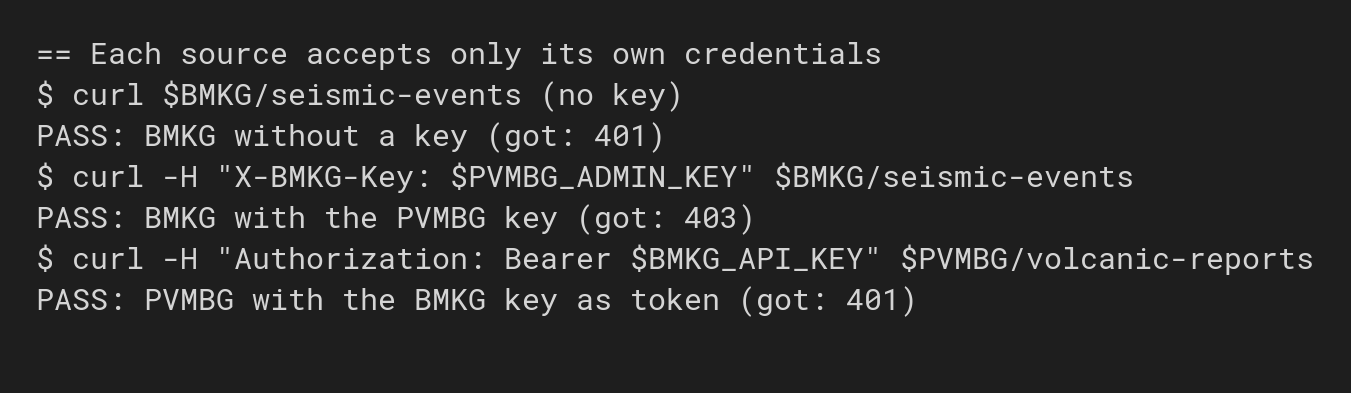
\includegraphics[width=\linewidth,height=0.72\textheight,keepaspectratio]{figures/bukti/viii1.png}
\caption{Kredensial satu instansi dipakai pada instansi lain}
\end{figure}

\subsection{Scope Media Ditolak Akses Field Mentah}

Akun Media hanya menerima field Ringkasan. Permintaan eksplisit terhadap field Mentah ditolak, sedangkan Operator menerima seluruh field.

\begin{figure}[H]
\centering
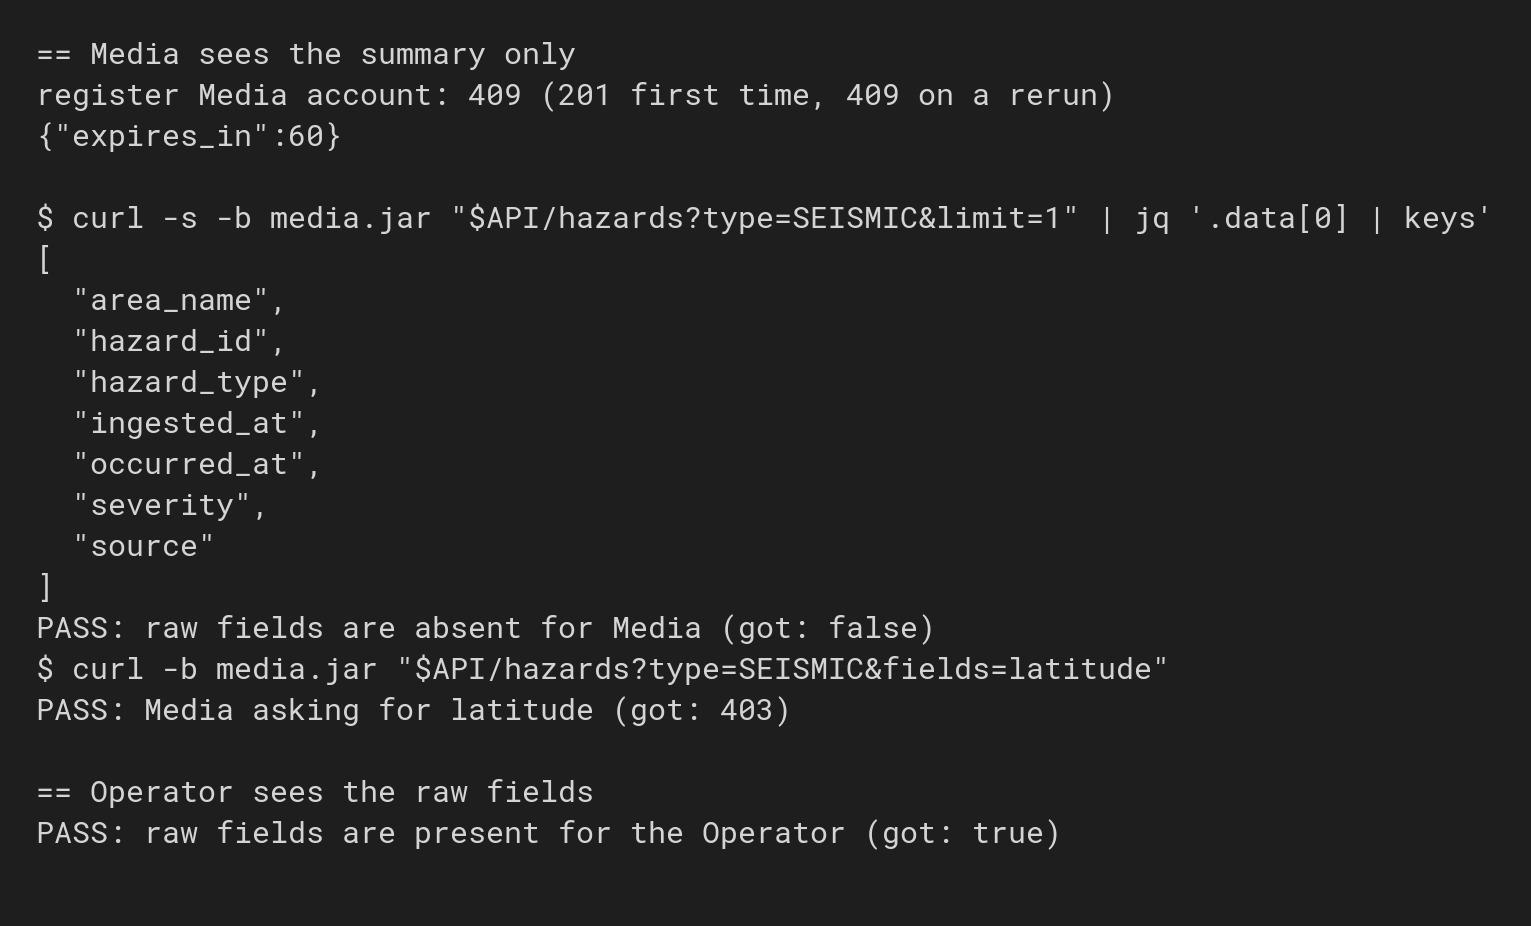
\includegraphics[width=\linewidth,height=0.72\textheight,keepaspectratio]{figures/bukti/viii2.png}
\caption{Field yang terlihat oleh Media dan Operator}
\end{figure}

\subsection{Token Expiry + Refresh Flow Tim Lapangan}

Akun Tim Lapangan login, skrip menunggu 65 detik sampai access token kedaluwarsa, lalu mengirim permintaan berikutnya. Respons 200 membawa cookie \texttt{jwt} dan \texttt{refresh\_token} baru, dan cookie lama ditolak setelah rotasi.

\begin{figure}[H]
\centering
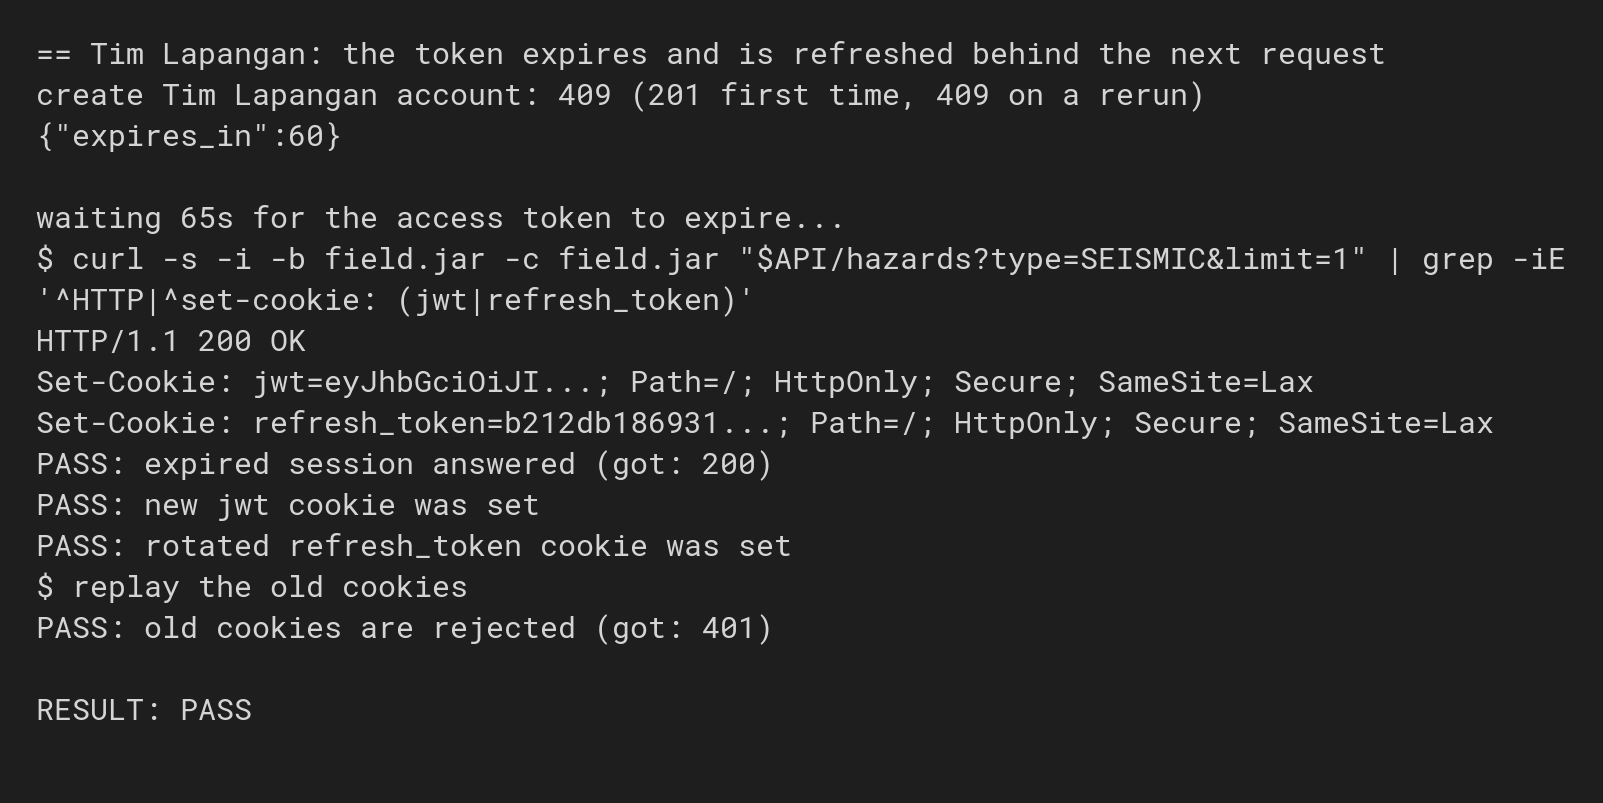
\includegraphics[width=\linewidth,height=0.72\textheight,keepaspectratio]{figures/bukti/viii3.png}
\caption{Kedaluwarsa token dan refresh Tim Lapangan}
\end{figure}

\subsection{Tidak Ada Hardcoded Credential}

Berkas \texttt{.env} berisi nilai asli tidak ikut ter-commit, sedangkan \texttt{.env.example} tersedia. Kode membaca rahasia dari \textit{environment variable}.

\begin{figure}[H]
\centering
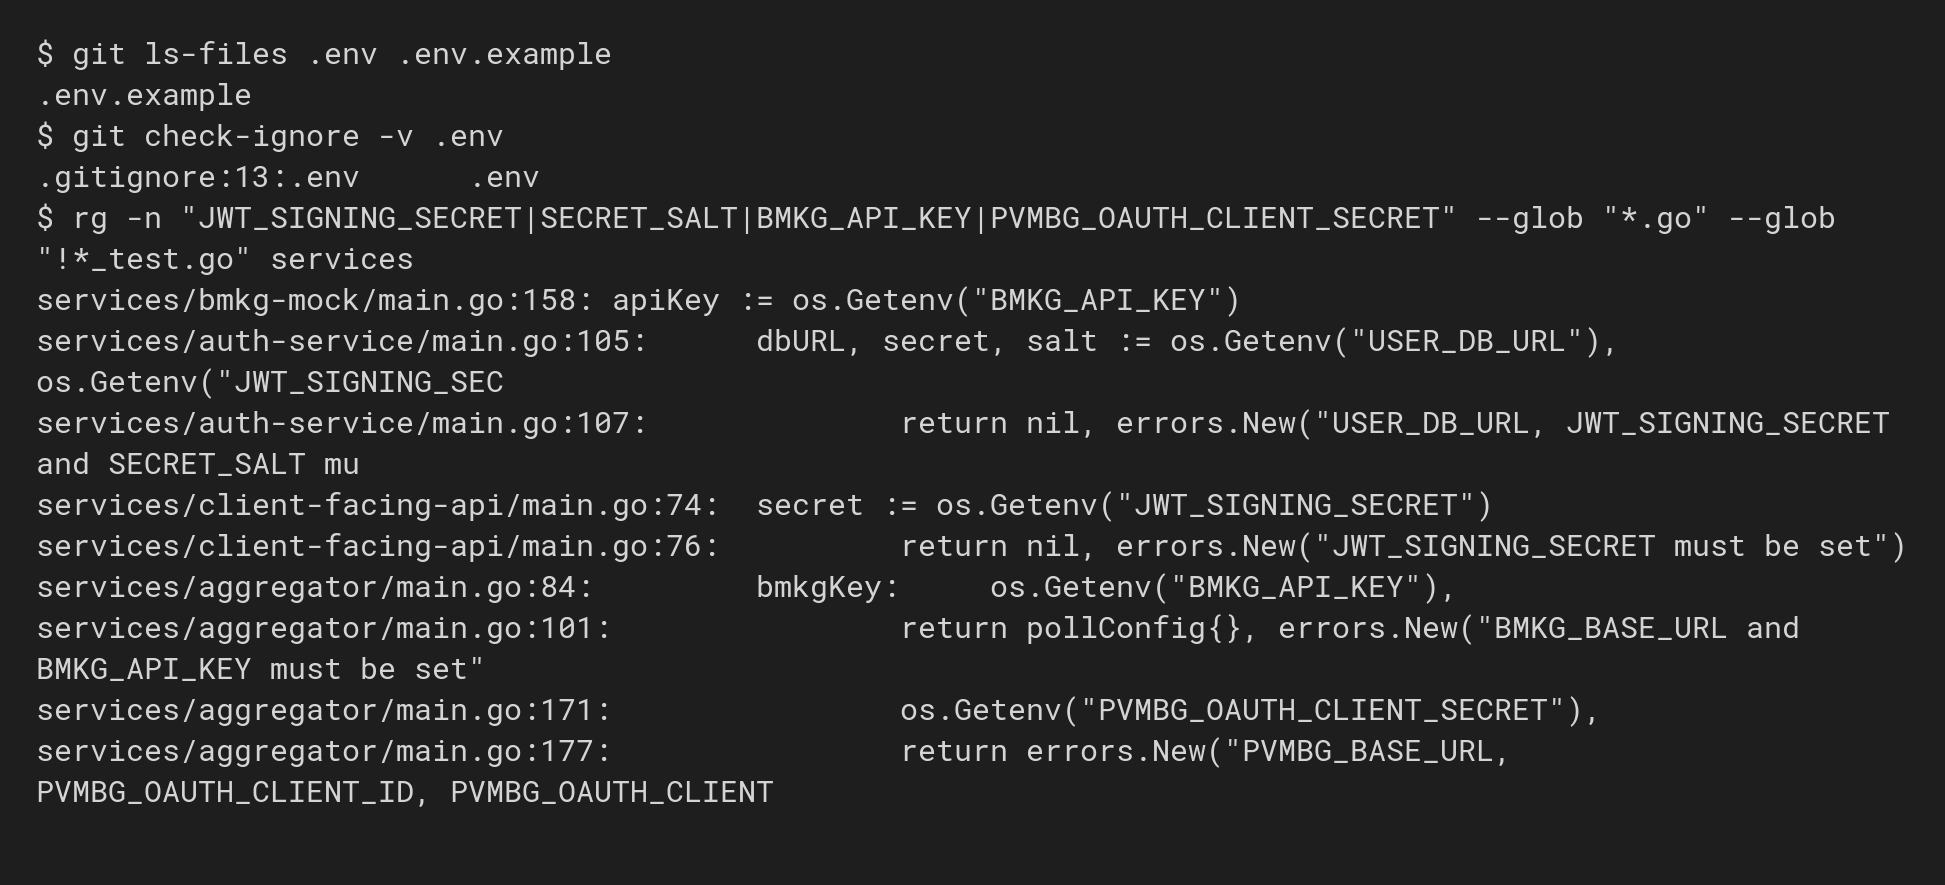
\includegraphics[width=\linewidth,height=0.72\textheight,keepaspectratio]{figures/bukti/viii4.png}
\caption{Pemeriksaan kredensial pada repositori}
\end{figure}

\section{Mekanisme yang Dipakai dan Alasan Tidak Membuka Celah Baru}

Mekanisme terbagi dua. Antara BNPB dan instansi sumber, BNPB mengikuti mekanisme masing-masing: \textit{API key} statis pada header \texttt{X-BMKG-Key} untuk BMKG, dan OAuth 2.0 dengan rotasi \textit{refresh token} untuk PVMBG. Antara \textit{client} dan BNPB, BNPB memakai IdP sendiri yang menerbitkan JWT HS256 dan \textit{refresh token} stateful, keduanya sebagai cookie \textit{HttpOnly}.

Alasan mekanisme ini tidak membuka celah baru adalah sebagai berikut.

\begin{itemize}
\item
  Kredensial tidak dapat dipakai lintas domain. Kunci BMKG ditolak oleh PVMBG dan token PVMBG ditolak oleh BMKG, dengan 401 atau 403. Tidak ada satu kunci pun yang dipakai untuk dua instansi maupun untuk \textit{client} di luar BNPB, sehingga kebocoran satu kredensial tidak membuka sumber lain.
\item
  Tiga \textit{client} adalah tiga identitas dan tiga akun berbeda dengan role tersimpan di User DB, bukan satu akun dengan \textit{flag}. Hak akses ditegakkan di Client-Facing API dari klaim JWT yang sudah diverifikasi: Media hanya menerima field Ringkasan, dan permintaan eksplisit terhadap field Mentah lewat parameter \texttt{fields} dijawab 403 tanpa memanggil Aggregator.
\item
  Token berumur pendek (60 detik secara default) dan \textit{refresh token} dirotasi pada setiap pemakaian, sehingga \textit{refresh token} lama ditolak setelah rotasi. Token curian hanya berguna sampai dipakai atau kedaluwarsa.
\item
  Cookie bertanda \textit{HttpOnly}, \textit{Secure}, dan \textit{SameSite}, sehingga tidak dapat dibaca JavaScript. Setiap 401 pada permintaan bercookie menghapus kedua cookie, karena browser tidak dapat menghapus cookie \textit{HttpOnly} sendiri.
\item
  Kegagalan login dijawab 401 tanpa menyebut email atau kata sandi mana yang salah. Login dan registrasi dibatasi per IP.
\item
  Rahasia tidak ada di kode. Kunci penandatangan JWT, \textit{salt}, kredensial OAuth, dan kunci API dibaca dari \textit{environment variable}, dan repositori hanya memuat \texttt{.env.example} berisi nilai contoh \texttt{change-me*}.
\item
  Aggregator tidak pernah menerbitkan atau menerima token \textit{client}, dan Canonical Store tidak dapat dijangkau dari jaringan mana pun selain milik Aggregator.
\end{itemize}

Batas dari pendekatan ini dicatat pada Batasan yang Disadari, terutama kepercayaan di tepi sistem dan kata sandi yang tidak diperkeras terhadap tebakan luring.
